\documentclass[tikz,border=5pt]{standalone}
\usepackage{amsmath,amssymb,bm}
\usetikzlibrary{arrows.meta,calc,decorations.markings}

\definecolor{accent}{RGB}{0, 100, 170}
\definecolor{highlight}{RGB}{200, 60, 30}
\definecolor{darkgreen}{RGB}{0, 120, 60}
\definecolor{earthblue}{RGB}{40,80,150}
\definecolor{orbitgray}{RGB}{100,100,100}

\begin{document}
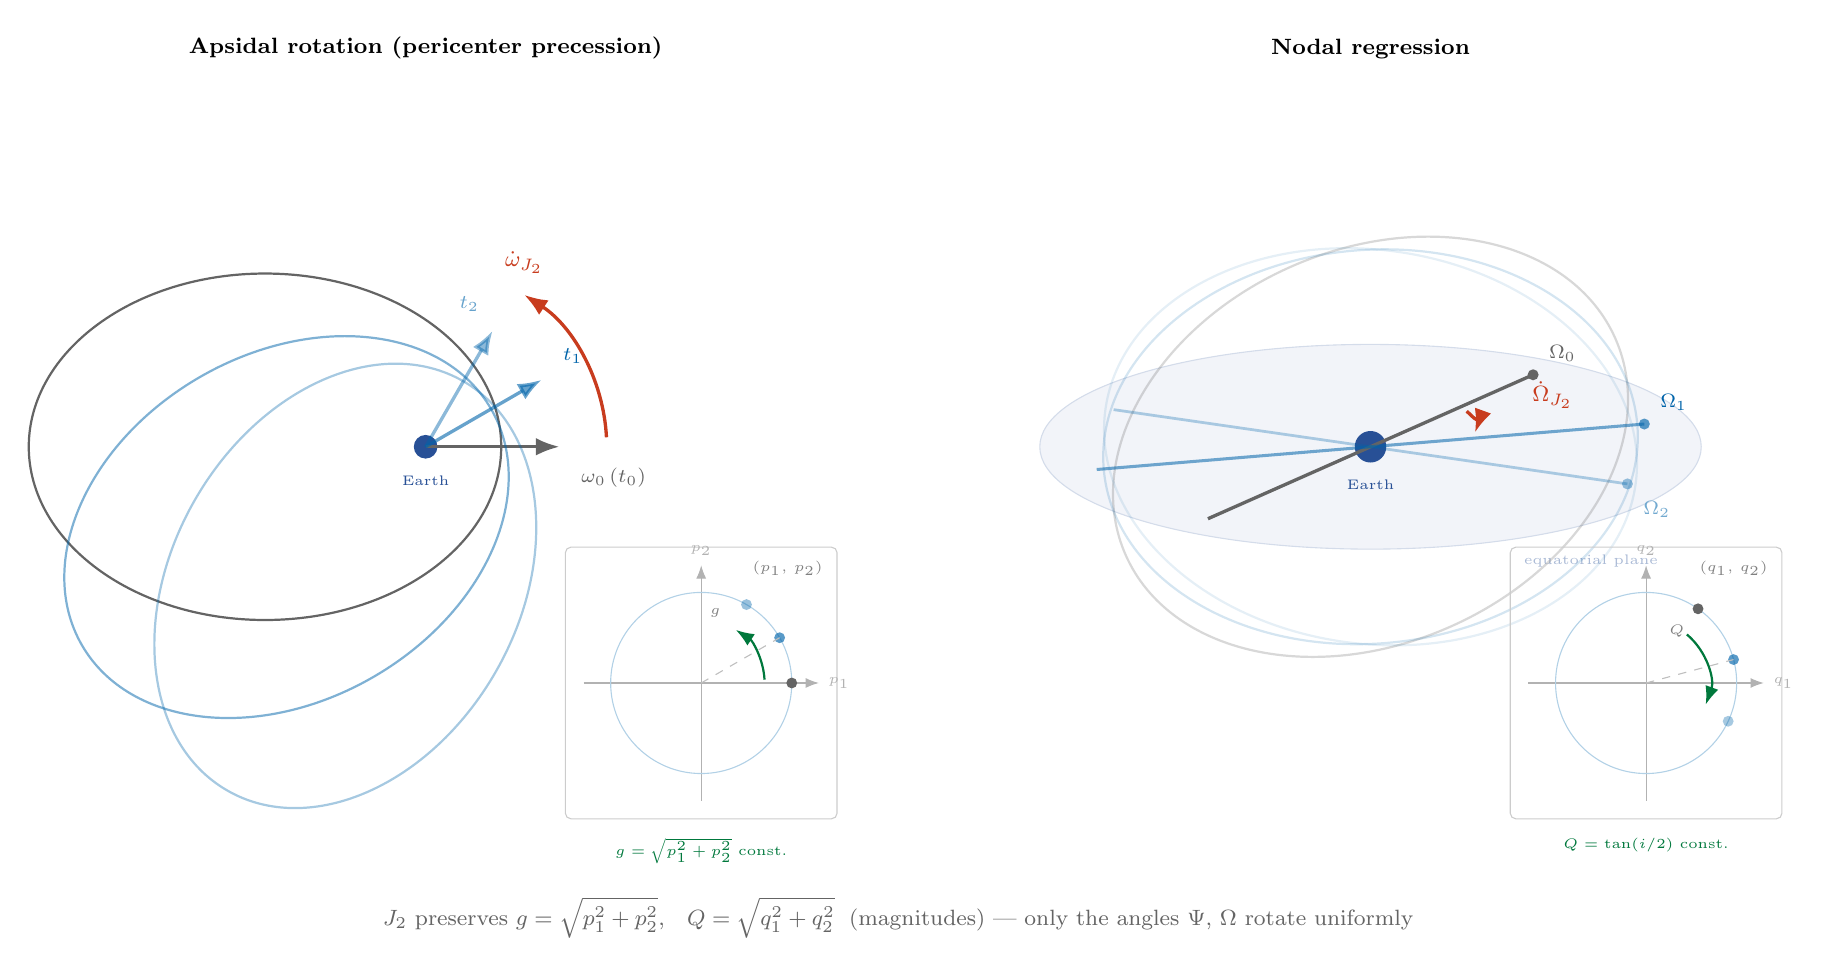
\begin{tikzpicture}[>=Latex, font=\small]

% =====================================================
% LEFT: Apsidal rotation (pericenter precession)
% =====================================================
\begin{scope}[shift={(-6,0)}]

  \node[font=\bfseries\footnotesize, anchor=south] at (0,4.8)
    {Apsidal rotation (pericenter precession)};

  % Earth at focus
  \fill[earthblue] (0,0) circle (0.15);
  \node[earthblue, font=\tiny, anchor=north] at (0,-0.25) {Earth};

  % Ellipse: a=3.0, b=2.2 => c=2.04, pericenter at a-c=0.96
  \def\eA{3.0}
  \def\eB{2.2}
  \def\eC{2.04}

  % Pericenter arrow length
  \def\arrowLen{1.7}

  % --- t0: omega=0 (orbitgray, full) ---
  \begin{scope}[rotate=0]
    \draw[orbitgray, thick] ({-\eC},0) ellipse [x radius=\eA, y radius=\eB];
    \draw[-{Latex[length=3mm]}, orbitgray, very thick]
      (0,0) -- (\arrowLen, 0);
  \end{scope}

  % --- t1: omega=30 (accent, moderate) ---
  \begin{scope}[rotate=30]
    \draw[accent, thick, opacity=0.50] ({-\eC},0) ellipse [x radius=\eA, y radius=\eB];
    \draw[-{Latex[length=3mm]}, accent, very thick, opacity=0.60]
      (0,0) -- (\arrowLen, 0);
  \end{scope}

  % --- t2: omega=60 (accent, more visible than before) ---
  \begin{scope}[rotate=60]
    \draw[accent, thick, opacity=0.35] ({-\eC},0) ellipse [x radius=\eA, y radius=\eB];
    \draw[-{Latex[length=3mm]}, accent, very thick, opacity=0.45]
      (0,0) -- (\arrowLen, 0);
  \end{scope}

  % Time/angle labels at the arrow tips — staggered to avoid overlap
  % t0 label below the arrow
  \node[orbitgray, font=\scriptsize, anchor=north west]
    at ({\arrowLen+0.15}, -0.15) {$\omega_0$\,($t_0$)};
  % t1 label above-right of the arrow
  \node[accent, font=\scriptsize, anchor=south west]
    at ({\arrowLen*cos(30)+0.15}, {\arrowLen*sin(30)+0.08}) {$t_1$};
  % t2 label to the left of the arrow tip
  \node[accent!60, font=\scriptsize, anchor=south east]
    at ({\arrowLen*cos(60)-0.05}, {\arrowLen*sin(60)+0.12}) {$t_2$};

  % Curved rotation arrow (radius well outside the arrow tips)
  \draw[->, highlight, very thick]
    ({2.3*cos(3)}, {2.3*sin(3)})
    arc[start angle=3, end angle=57, radius=2.3];
  \node[highlight, font=\footnotesize, anchor=south]
    at ({2.3*cos(57)}, {2.3*sin(57)+0.15}) {$\dot{\omega}_{J_2}$};

  % ===== INSET: (p1, p2) circle =====
  \begin{scope}[shift={(3.5,-3.0)}, scale=1.15]
    \draw[gray!40, thin, rounded corners=2pt] (-1.5,-1.5) rectangle (1.5,1.5);

    \draw[->, gray!60, thin] (-1.3,0) -- (1.3,0) node[right, font=\tiny] {$p_1$};
    \draw[->, gray!60, thin] (0,-1.3) -- (0,1.3) node[above, font=\tiny] {$p_2$};

    \draw[accent!30] (0,0) circle (1.0);

    \fill[orbitgray] ({1.0*cos(0)}, {1.0*sin(0)}) circle (0.06);
    \fill[accent, opacity=0.65] ({1.0*cos(30)}, {1.0*sin(30)}) circle (0.06);
    \fill[accent, opacity=0.40] ({1.0*cos(60)}, {1.0*sin(60)}) circle (0.06);

    \draw[->, darkgreen, thick]
      ({0.7*cos(3)}, {0.7*sin(3)})
      arc[start angle=3, end angle=57, radius=0.7];

    \draw[gray!50, thin, dashed] (0,0) -- ({1.0*cos(30)}, {1.0*sin(30)});
    \node[font=\tiny, gray, anchor=south east] at (0.32, 0.62) {$g$};

    \node[font=\tiny, gray, anchor=north east] at (1.45,1.45) {$(p_1,\, p_2)$};
  \end{scope}

  \node[font=\tiny, darkgreen, anchor=north] at (3.5, -4.85)
    {$g = \sqrt{p_1^2 + p_2^2}$ const.};

\end{scope}

% =====================================================
% RIGHT: Nodal regression
% =====================================================
\begin{scope}[shift={(6,0)}]

  \node[font=\bfseries\footnotesize, anchor=south] at (0,4.8)
    {Nodal regression};

  % Equatorial plane
  \fill[earthblue!6] (0,0) ellipse [x radius=4.2, y radius=1.3];
  \draw[earthblue!20, thin] (0,0) ellipse [x radius=4.2, y radius=1.3];
  \node[earthblue!40, font=\tiny, anchor=north] at (2.8, -1.25) {equatorial plane};

  % Earth
  \fill[earthblue] (0,0) circle (0.2);
  \node[earthblue, font=\tiny, anchor=north] at (0,-0.3) {Earth};

  \def\nodeLen{3.6}
  \def\foreshort{0.31}

  % --- t0: Omega=55 ---
  \pgfmathsetmacro{\nAx}{\nodeLen*cos(55)}
  \pgfmathsetmacro{\nAy}{\nodeLen*sin(55)*\foreshort}
  \draw[orbitgray, thick, line width=1.2pt]
    ({-\nAx},{-\nAy}) -- ({\nAx},{\nAy});
  \fill[orbitgray] ({\nAx},{\nAy}) circle (0.07);
  \node[orbitgray, font=\scriptsize, anchor=south west]
    at ({\nAx+0.08},{\nAy+0.05}) {$\Omega_0$};
  \pgfmathsetmacro{\tiltA}{atan2(\nAy, \nAx)}
  \begin{scope}[rotate=\tiltA]
    \draw[orbitgray, thick, opacity=0.25]
      (0,0) ellipse [x radius=3.4, y radius=2.5];
  \end{scope}

  % --- t1: Omega=15 ---
  \pgfmathsetmacro{\nBx}{\nodeLen*cos(15)}
  \pgfmathsetmacro{\nBy}{\nodeLen*sin(15)*\foreshort}
  \draw[accent, thick, opacity=0.55, line width=1.1pt]
    ({-\nBx},{-\nBy}) -- ({\nBx},{\nBy});
  \fill[accent, opacity=0.65] ({\nBx},{\nBy}) circle (0.07);
  \node[accent, font=\scriptsize, anchor=south west]
    at ({\nBx+0.08},{\nBy+0.05}) {$\Omega_1$};
  \pgfmathsetmacro{\tiltB}{atan2(\nBy, \nBx)}
  \begin{scope}[rotate=\tiltB]
    \draw[accent, thick, opacity=0.17]
      (0,0) ellipse [x radius=3.4, y radius=2.5];
  \end{scope}

  % --- t2: Omega=-25 ---
  \pgfmathsetmacro{\nCx}{\nodeLen*cos(-25)}
  \pgfmathsetmacro{\nCy}{\nodeLen*sin(-25)*\foreshort}
  \draw[accent, thick, opacity=0.30, line width=1.0pt]
    ({-\nCx},{-\nCy}) -- ({\nCx},{\nCy});
  \fill[accent, opacity=0.4] ({\nCx},{\nCy}) circle (0.07);
  \node[accent!55, font=\scriptsize, anchor=north west]
    at ({\nCx+0.08},{\nCy-0.1}) {$\Omega_2$};
  \pgfmathsetmacro{\tiltC}{atan2(\nCy, \nCx)}
  \begin{scope}[rotate=\tiltC]
    \draw[accent, thick, opacity=0.10]
      (0,0) ellipse [x radius=3.4, y radius=2.5];
  \end{scope}

  % Regression arrow
  \draw[->, highlight, very thick]
    ({1.9*cos(50)}, {1.9*sin(50)*\foreshort})
    arc[start angle={atan2(sin(50)*\foreshort, cos(50))},
        end angle={atan2(sin(-20)*\foreshort, cos(-20))},
        x radius=1.9, y radius={1.9*\foreshort}];
  \node[highlight, font=\footnotesize, anchor=south west]
    at ({2.0*cos(15)}, {2.0*sin(15)*\foreshort + 0.2}) {$\dot{\Omega}_{J_2}$};

  % ===== INSET: (q1, q2) circle =====
  \begin{scope}[shift={(3.5,-3.0)}, scale=1.15]
    \draw[gray!40, thin, rounded corners=2pt] (-1.5,-1.5) rectangle (1.5,1.5);

    \draw[->, gray!60, thin] (-1.3,0) -- (1.3,0) node[right, font=\tiny] {$q_1$};
    \draw[->, gray!60, thin] (0,-1.3) -- (0,1.3) node[above, font=\tiny] {$q_2$};

    \draw[accent!30] (0,0) circle (1.0);

    \fill[orbitgray] ({1.0*cos(55)}, {1.0*sin(55)}) circle (0.06);
    \fill[accent, opacity=0.65] ({1.0*cos(15)}, {1.0*sin(15)}) circle (0.06);
    \fill[accent, opacity=0.35] ({1.0*cos(-25)}, {1.0*sin(-25)}) circle (0.06);

    \draw[->, darkgreen, thick]
      ({0.7*cos(50)}, {0.7*sin(50)})
      arc[start angle=50, end angle=-20, radius=0.7];

    \draw[gray!50, thin, dashed] (0,0) -- ({1.0*cos(15)}, {1.0*sin(15)});
    \node[font=\tiny, gray, anchor=south west] at (0.15, 0.4) {$Q$};

    \node[font=\tiny, gray, anchor=north east] at (1.45,1.45) {$(q_1,\, q_2)$};
  \end{scope}

  \node[font=\tiny, darkgreen, anchor=north] at (3.5, -4.85)
    {$Q = \tan(i/2)$ const.};

\end{scope}

% =====================================================
% BOTTOM ANNOTATION
% =====================================================
\node[font=\footnotesize, anchor=north, text=orbitgray, align=center] at (0, -5.6)
  {$J_2$ preserves $g = \sqrt{p_1^2+p_2^2}$, \;
   $Q = \sqrt{q_1^2+q_2^2}$ \;(magnitudes)
   --- only the angles $\Psi$, $\Omega$ rotate uniformly};

\end{tikzpicture}
\end{document}
